\subsection{Relative droplets kinematics  }

In the previous sections we have seen that the timescale governing both the microstructure evolution and the droplet pair relative velocity is $\tau_p$.   
We now give a visual representation of the nearest-pair relative velocity in space to better understand how the relative kinematics   behave.  
To that end we compute the nearest relative velocity and age, averaged on all ages, that is,
\begin{align*}
    \textbf{w}^\text{r}_pP_r(\textbf{x},\textbf{r},t)
    =\int_0^\infty \textbf{w}^\text{nst}_pP_\text{nst}(\textbf{x},\textbf{r},t,a) da,\\
    a^rP_r(\textbf{x},\textbf{r},t)
    =\int_0^\infty a P_\text{nst}(\textbf{x},\textbf{r},t,a) da.
\end{align*}
The superscript $^\text{r}$ indicates that the quantity $\textbf{w}^\text{r}_p$ and $a^r$ is conditioned on the relative position \textbf{r} only.
As will be demonstrated, having a good estimation of these velocities and ages mean fields allows one to reconstruct the history and kinematics   of the droplets interactions. 
To be able to visualize
$\textbf{w}^\text{r}_p(\textbf{x},\textbf{r},t)$
and 
$a^r(\textbf{x},\textbf{r},t)$
on 2D plots, we consider an axis of symmetry along the vertical axis and average the values of 
$\textbf{w}^\text{r}_p(\textbf{x},\textbf{r},t)$
and $a^r(\textbf{x},\textbf{r},t)$
on the polar coordinate, as has been done for $P_\text{nst}$ in \ref{sec:microstructure}. 
However, unlike in \ref{sec:microstructure} we do not assume symmetry with respect to the horizontal plane. 

\subsubsection{Impact of the inertial effects}

The first effect that we study is the impact of inertia on the droplets' relative kinematics.    
In \ref{fig:Why_Ga_matter} we display the velocity fields $\textbf{w}_p^r$ represented by the arrows that are colored by the mean dimensionless age $a^r$.  
On the left panel, we display a low inertia case ($Ga = 10$), while on the right panel, we display a high inertia case ($Ga=100$), both for $\lambda =1$ and $\phi=0.05$.
\begin{figure}[h!]
    \centering
    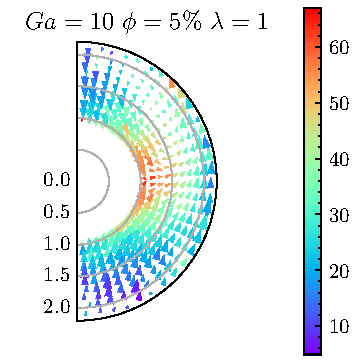
\includegraphics[height=0.35\textwidth]{image/HOMOGENEOUS_NEW/Dist/U_rel_l_1_Ga_10_PHI_5.pdf}
    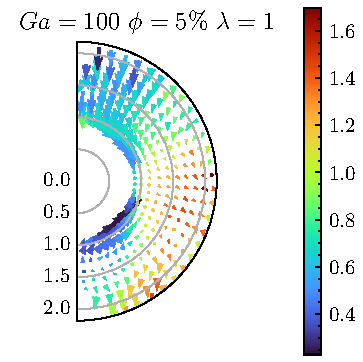
\includegraphics[height=0.35\textwidth]{image/HOMOGENEOUS_NEW/Dist/U_rel_l_1_Ga_100_PHI_5.pdf}
    % \begin{tikzpicture}[scale=0.8]
    %     \filldraw[ gray!50!white](0,0) circle (0.5);
    %     \filldraw[ gray!50!white](1,3)circle (0.5);
    %     \filldraw[ gray!50!white](-0.2,3.5)circle (0.5);
    %     % \draw[fill=gray,opacity=0.2](5,-0.2)circle (0.5);
    %     % \draw[fill=gray,opacity=0.2](-3,2)circle (0.5);
    %     % \draw[fill=gray,opacity=0.2](-5,0.2)circle (0.5);
    %     \draw(0,0)node[right]{$p_1, \; \textbf{x} = 0 $};
    %     \draw[dashed](0,0)--(1,3)node[right]{$p_2, \;\textbf{x}+\textbf{r}$};
    %     \draw[dashed](-0.2,3.5)node[right]{$p_3$};
    % \end{tikzpicture} 
    % 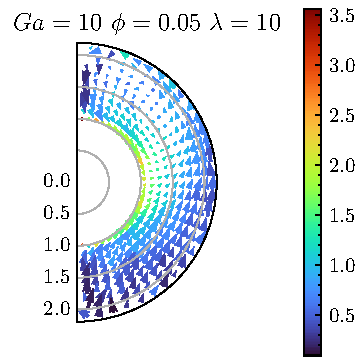
\includegraphics[height=0.35\textwidth]{image/HOMOGENEOUS_NEW/Dist/U_rel_l_10_Ga_10_PHI_5.pdf}
    % 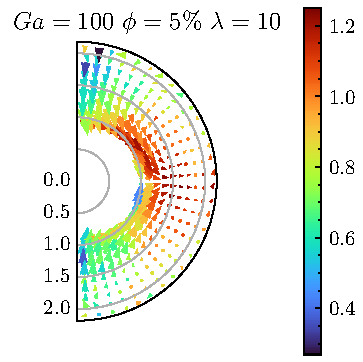
\includegraphics[height=0.35\textwidth]{image/HOMOGENEOUS_NEW/Dist/U_rel_l_10_Ga_100_PHI_5.pdf}
    \caption{
         Quiver plots of the relative averaged velocity field $\textbf{w}^\text{r}(\textbf{x},\textbf{r},t)$ colored by the averaged dimensionless age $a^r(\textbf{x},\textbf{r},t)$ for $\phi = 0.05$ and $\lambda +1$.
         (left) $Ga = 10$ (right) $Ga =100$. }
    \label{fig:Why_Ga_matter}
\end{figure}

The first aspect that we would like to clarify is the non-fore-aft symmetry of the velocity fields $\textbf{w}_p^\text{nst}$ with respect to the horizontal plane. 
% Indeed, in plots displayed on \ref{fig:Why_Ga_matter} we remark that the $\textbf{w}_p^\text{nst}$ exhibit a clear asymmetry with respect to the horizontal plane.
This is explained by the non commutativity of the function $h_{ij}$ in the indices $i$ and $j$ in \ref{eq:q_nstij}, as a result $\textbf{w}_p^r(\textbf{x},t,r,\theta) \neq \textbf{w}_p^r(\textbf{x},t,r,-\theta)$. 
Indeed, as it is depicted on \ref{fig:diagram_asym}, in the cases where the neighboring nearest droplet is far from the test droplet, the chance for this droplet to have another nearest neighbor which is closer is high. 
Thus, the nearest neighbor of the nearest neighbor of the test droplet, is not necessarily the test droplet. 
This induces an asymmetry in the nearest neighbor statistics. 
That explains why the plots on \ref{fig:Why_Ga_matter} are not symmetric when we observe the fields at sufficiently large distance $|\textbf{r}|$. 
Note that this asymmetry would not be present if we had considered classical particle pair average as done in \cite{shajahan2023inertial}. 

To summarize, in the situation where we observe $\textbf{w}_p^r$ for large $|\textbf{r}|$ the test droplet can be considered as being \textit{isolated}, as its nearest neighbor is at a large distance $|\textbf{r}|$ from the test droplet. 
Additionally, the nearest neighboring droplet, if located far enough, has 
potentially a nearest neighbor that is closer than the test sphere, as explained on \ref{fig:diagram_asym}. 
Consequently, provided that the nearest neighbor of the test sphere is far enough, we can be sure that on average it approaches a pair of droplets or more, that are packed together. 

\begin{figure}[h!]
    \centering
    \hfill
    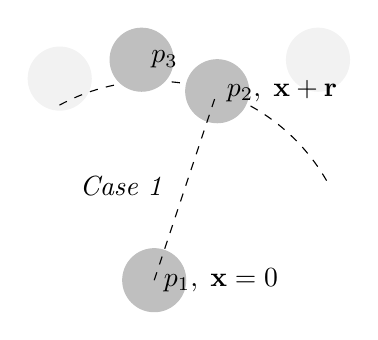
\begin{tikzpicture}[scale=0.8]
        \filldraw[ gray!10!white](+2.6,3.5)circle (0.5);
        \filldraw[ gray!10!white](-1.5,3.2)circle (0.5);
        \draw[dashed](30:3.16) arc (30:120:3.16);
        \filldraw[ gray!50!white](0,0) circle (0.5);
        \filldraw[ gray!50!white](1,3)circle (0.5);
        \filldraw[ gray!50!white](-0.2,3.5)circle (0.5);
        \draw(0,0)node[right]{$p_1, \; \textbf{x} = 0 $};
        \draw[dashed](0,0)--(1,3)node[right]{$p_2, \;\textbf{x}+\textbf{r}$};
        \draw[dashed](-0.2,3.5)node[right]{$p_3$};
        \node[ultra thick] (title) at (-0.5,1.5) {\textit{Case 1}};
    \end{tikzpicture} 
    \hfill
    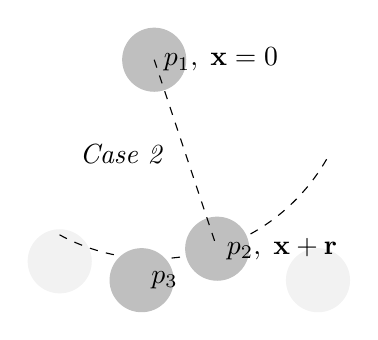
\begin{tikzpicture}[rotate=180, xscale=-0.8,yscale=0.8]
        \filldraw[ gray!10!white](+2.6,3.5)circle (0.5);
        \filldraw[ gray!10!white](-1.5,3.2)circle (0.5);
        \draw[dashed](30:3.16) arc (30:120:3.16);
        \filldraw[ gray!50!white](0,0) circle (0.5);
        \filldraw[ gray!50!white](1,3)circle (0.5);
        \filldraw[ gray!50!white](-0.2,3.5)circle (0.5);
        \draw(0,0)node[right]{$p_1, \; \textbf{x} = 0 $};
        \draw[dashed](0,0)--(1,3)node[right]{$p_2, \;\textbf{x}+\textbf{r}$};
        \draw[dashed](-0.2,3.5)node[right]{$p_3$};
        \node[ultra thick] (title) at (-0.5,1.5) {\textit{Case 2}};
    \end{tikzpicture} 
    \hfill
    % \begin{tikzpicture}[scale=0.8]
    %     \filldraw[ gray!10!white](+2.6,3.5)circle (0.5);
    %     \filldraw[ gray!10!white](-1.5,3.2)circle (0.5);
    %     \draw[dashed](-30:3.16) arc (-30:-120:3.16);
    %     \filldraw[ gray!50!white](0,0) circle (0.5);
    %     \filldraw[ gray!50!white](1,-3)circle (0.5);
    %     % \filldraw[ gray!20!white](-1.4,-3.3)circle (0.5);
    %     \filldraw[ gray!50!white](-0.2,-3.5)circle (0.5);
    %     % \draw[fill=gray,opacity=0.2](5,-0.2)circle (0.5);
    %     % \draw[fill=gray,opacity=0.2](-3,2)circle (0.5);
    %     % \draw[fill=gray,opacity=0.2](-5,0.2)circle (0.5);
    %     \draw(0,0)node[right]{$p_1, \; \textbf{x} = 0 $};
    %     \draw[dashed](0,0)--(1,-3)node[right]{$p_2, \;\textbf{x}+\textbf{r}$};
    %     \draw[dashed](-0.2,-3.5)node[right]{$p_3$};
    %     \node[ultra thick] (title) at (-0.5,-1.5) {$Case\; 2$};
    % \end{tikzpicture} 
    \caption{
        Diagram that highlights the asymmetry of the nearest pair statistics when the nearest neighbor is relatively far from the test particle.
        (\textit{Case 1}) droplet $p_1$ with  its nearest neighbor, $p_2$, located at the \underline{top} of it. 
        (\textit{Case 2}) droplet $p_1$ with  its nearest neighbor, $p_2$, located at the \underline{bottom} of it. 
        (\textit{Case 1} and \textit{2})
        In these situations, the droplet $p_2$ located at $\textbf{x} + \textbf{r}$, is the nearest neighbor of the droplet $p_1$ located at $\textbf{x}$. 
        Since $|\textbf{r}|/d$ is assumed to be large, the nearest neighbor of the droplet $p_2$ is more likely to be another nearest neighbor than $p_1$ such as the droplet $p_3$, which is closer.
        This is due to the rapid decay of $P_\text{nst}$ for large $|\textbf{r}|/d$, see \ref{fig:Pnst_high_Ga}. 
        In these cases, the nearest neighbor of $p_1$ is $p_2$, but the contrary is not true, inducing asymmetry in the statistics.  
    }
    \label{fig:diagram_asym}
\end{figure}

Now that this issue has been clarified, we can proceed to interpret the plots in \ref{fig:Why_Ga_matter}.
The beginning of the interactions happens at the early ages, meaning in the dark blue areas in  \ref{fig:Why_Ga_matter}, which are located on the top or bottom of the droplet of reference.
The ending of the interactions corresponds to the greater ages, which are represented by the red areas. 
As shown by \ref{fig:Why_Ga_matter} (left), at low \textit{Galileo} number the nearest droplet has a tendency to come from the top or bottom and leave through the sides. 
If the nearest droplet is at a reasonable distance $|\textbf{r}| < 1.5d$ on the sides of the test droplet, we can see that the vertical relative velocity is on average zero, but positive in the radial component.
In this area, the age is at its maximum (dark red zone), therefore the interactions come to an end, meaning that the nearest droplets get replaced by another. 
Note that the droplets at a larger distance of the test droplet, say $|\textbf{r}|>2$, have an averaged positive vertical relative velocity. 
As discussed above, in this situation the neighbor on the side is more likely to be closer to another droplet. 
Consequently, if the test droplet is isolated, with neighboring droplets sufficiently far on the side, it will rise on average with a lower velocity than the latter droplets.
Thus, droplets at contact seem to get apart because of the non-zero radial velocity, and droplets at a distance seem to get apart because of the non-zero vertical velocity.  
Consequently, on average the side-by-side configuration is not stable in this case, which partly explains why the droplet distribution doesn't form any layer or such oriented microstructure at these $Ga$.   

% A plausible explanation for this phenomenon is that the leading droplet accelerate the trailing droplet with its wake on a first stage. 
% Then, the trailing droplet arise to the same altitude as the leading droplet, but still goes faster than the leading droplet due to the acceleration provided by the wake of the latter droplet.
% If the droplets get in contact then the interaction duration seem to last longer, and the droplets might even get trap in a small stagnation zone on the side of the droplets.


For high \textit{Galileo} numbers, see \ref{fig:Why_Ga_matter} (right), the relative averaged velocity is nearly zero on the sides and below the test droplet. 
It is a statistical representation, meaning that, $\textbf{w}_p^r = 0$, indicates that the droplets relative  velocities are not correlated with the relative position in this area. 
Thus, it is hard to say if the area where $\textbf{w}_p^r = 0$ corresponds to actual stagnation zones where both droplets are in equilibrium, or if the relative velocity is just not correlated. 

The droplets at a large distance on the top of the test droplet have a downward velocity. 
This means that if the test sphere is isolated and approaches one or several  droplets on top of it (see \ref{fig:diagram_asym} (\textit{Case 1})), it will eventually catch up the latter droplets. 
On the contrary, if the droplet is isolated and the nearest neighbor is at the bottom (see \ref{fig:diagram_asym} (\textit{Case 2})), the velocity is either pointing downward, or it is not correlated with the position, as indicated by the magnitude of $\textbf{w}_p^r$. 
A plausible explanation for this phenomenon is that the reference droplet, when being isolated, goes faster than the potentially packed nearest neighbor.
Therefore, the test sphere can either catch up with the nearest droplet if it is above, or move further away from it if it is below.
Also, it is interesting to note that in this case the droplets at near contact on the bottom of the test droplet result from early interaction, denoted by the dark blue zone. 
It can be interpreted as follows: since 
initial duration of interaction is on average low in this zone, it does mean that droplets replace an old nearest neighbor that were at near contact with the test droplets. 
Thus, in this case, the nearest neighbor reaches the test sphere which was rising slowly because of a potentially closer neighbor. 

Ultimately, the fields $\textbf{w}^r_p(\textbf{x},\textbf{r}, a)$ provide a quantitative averaged representation of what is known as the \textit{Drafting Kissing Tumbling} \citep{fortes1987nonlinear} mechanism. 
Indeed, in both cases droplets eventually approach vertically (\textit{Drafting}), nearly touch each other (\textit{Kissing}), and leave through the sides (\textit{Tumbling}). 
Statistically, the \textit{Tumbling} part is not present in the high inertia case, which explains the creation of anisotropic structures or more stable side-by-side configurations. 
For bubble pair interactions \citet{zhang2021three} observed such DKT behavior.
They also reported side-by-side stable configurations of pairs. 
However, at the same \textit{Galileo} as \citet{zhang2021three} ($Ga = 10$) we were not able to identify this mechanism. 


To support the observations made above, we displayed in \ref{fig:unst_ga} the absolute conditioned averaged center of mass velocity of the test sphere, defined as,
\begin{equation*}
    \textbf{u}^\text{r}_p(\textbf{x},\textbf{r},t)  
    =
    \frac{1}{P_r(\textbf{x},\textbf{r},t)}
    \int_0^\infty \textbf{u}^\text{nst}_pP_\text{nst}(\textbf{x},\textbf{r},t,a) da
\end{equation*}
In \ref{fig:unst_ga} (left) we see that the magnitude of the test droplet's vertical velocity is higher than the droplet phase vertical velocity $\textbf{u}_p$ when the nearest neighbor is at near contact to the test droplet, either above or below.
\begin{figure}[h!]
    \centering
    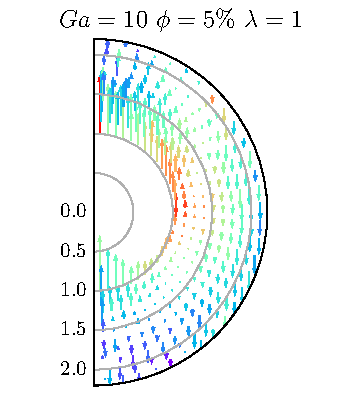
\includegraphics[height=0.35\textwidth]{image/HOMOGENEOUS_NEW/Dist/U_l_1_Ga_10_PHI_5.pdf}
    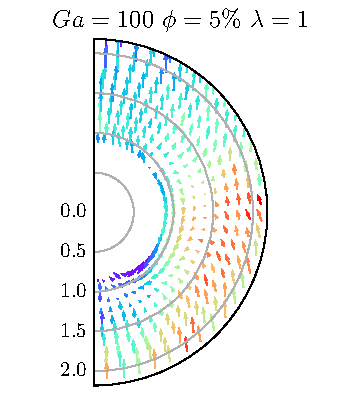
\includegraphics[height=0.35\textwidth]{image/HOMOGENEOUS_NEW/Dist/U_l_1_Ga_100_PHI_5.pdf}
    \caption{
         Quiver plots of the conditioned droplet velocity field $\textbf{u}^\text{r}(\textbf{x},\textbf{r},t)$ colored by the averaged dimensionless vertical velocity difference : $(\textbf{u}^\text{r} - \textbf{u}_p )/ \textbf{u}_p$, for $\lambda = 1$ and $\phi = 0.05$. 
         (left) Low \textit{Galileo} number $Ga = 10$.
        (right) High \textit{Galileo} number $Ga = 100$.
         }
    \label{fig:unst_ga}
\end{figure}
When the nearest neighbor is at a large distance from the test droplet, its average velocity is lower than $\textbf{u}_p$. 
When inertia is high, however, the test droplet velocity is higher when being isolated than with its neighbor at near contact. 
Additionally, we can see that when the droplet is on the side at near contact or below, the test sphere's velocity  is lower than the mean. 
In brief in the case of $Ga = 10$ it seems that isolated droplets rise slower than close neighbors packed together. 
While at higher \textit{Galileo} number it is the opposite, we observe that isolated droplets go faster than packed neighbors. 


\subsubsection{The volume fraction dependency}
As observed in \ref{fig:A} the effect of increasing $\phi$ is that it makes the droplet distribution slightly more isotropic for $\phi >0.1$. 
\begin{figure}[h!]
    \centering
    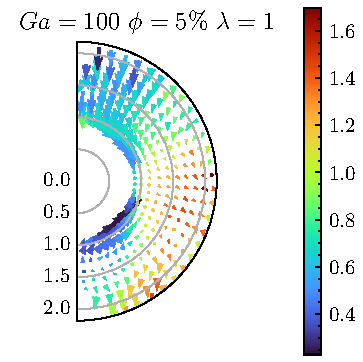
\includegraphics[height=0.35\textwidth]{image/HOMOGENEOUS_NEW/Dist/U_rel_l_1_Ga_100_PHI_5.pdf}
    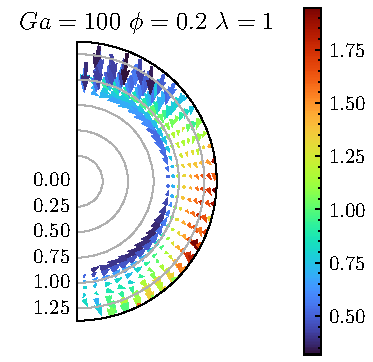
\includegraphics[height=0.35\textwidth]{image/HOMOGENEOUS_NEW/Dist/U_rel_l_1_Ga_100_PHI_20.pdf}
    % 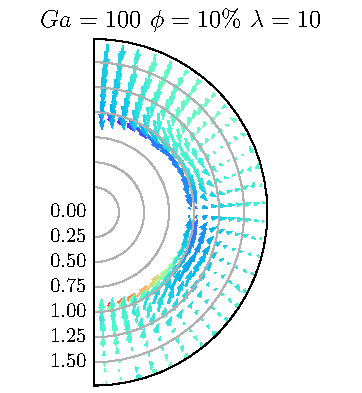
\includegraphics[height=0.35\textwidth]{image/HOMOGENEOUS_NEW/Dist/U_rel_l_10_Ga_100_PHI_10.pdf}
    % 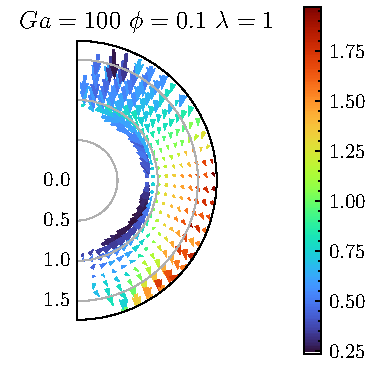
\includegraphics[height=0.35\textwidth]{image/HOMOGENEOUS_NEW/Dist/U_rel_l_1_Ga_100_PHI_10.pdf}
    \caption{Quiver plots of the relative averaged velocity field $\textbf{w}^\text{r}(\textbf{x},\textbf{r},t)$ colored by the averaged dimensionless age $a^r(\textbf{x},\textbf{r},t)$, for $Ga = 100$ and $\lambda = 1$. 
    (left) Low \textit{Galileo} number $\phi = 0.05$.
    (right) High \textit{Galileo} number $\phi = 0.2$. }
    \label{fig:Why_Phi_matter}
\end{figure}
In \ref{fig:Why_Phi_matter} we expose two situations with various volume fractions. 
In both graphs, we observe the same trend, despite the changes in length scales, which are due to the variations in volume fraction. 
Indeed, the stagnation zones with dark red color and the droplet having short ages, dark blue color, are located approximately at the same location. 
We still observe the fore-aft asymmetry with respect to the horizontal plane, as was discussed above. 
For other $\lambda$ and $Ga$ no particular differences can be observed with varying $\phi$. 
Overall, even if small differences may be present, the change in volume fraction doesn't seem to affect the relative kinematics   of interaction between droplets. 

\subsubsection{Influence of the viscosity ratio}

Lastly, we turn our attention to the effect of the viscosity ratio on pair relative kinematics. 
The question that we are trying to answer is : why does a smaller viscosity ratio increase the anisotropy of the tensor $\textbf{R}(\textbf{x},t)$ as shown in \ref{fig:A}. 
With this objective in mind, we compare two cases at $Ga = 100$ and $\phi =0.05$, where we observe a clear difference between the distributions (see \ref{fig:Pnst_high_Ga}) between $\lambda = 1$ and $\lambda = 10$.
\begin{figure}[h!]
    \centering
    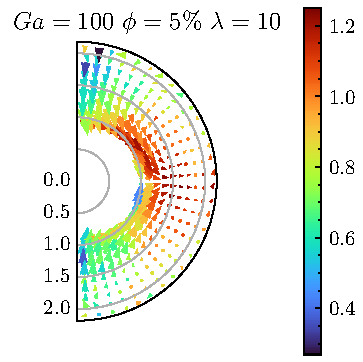
\includegraphics[height=0.35\textwidth]{image/HOMOGENEOUS_NEW/Dist/U_rel_l_10_Ga_100_PHI_5.pdf}
    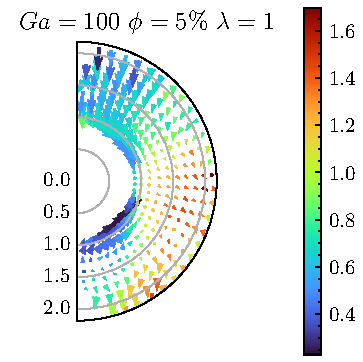
\includegraphics[height=0.35\textwidth]{image/HOMOGENEOUS_NEW/Dist/U_rel_l_1_Ga_100_PHI_5.pdf}
    % 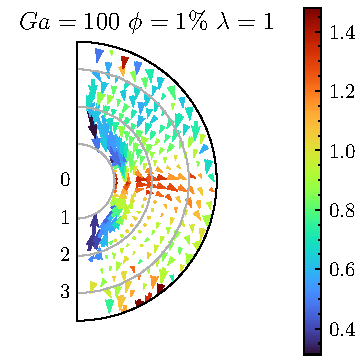
\includegraphics[height=0.35\textwidth]{image/HOMOGENEOUS_NEW/Dist/U_rel_l_1_Ga_100_PHI_1.pdf}
    % 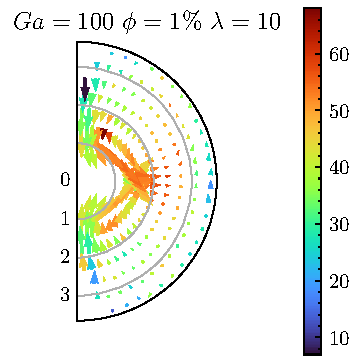
\includegraphics[height=0.35\textwidth]{image/HOMOGENEOUS_NEW/Dist/U_rel_l_10_Ga_100_PHI_1.pdf}
    \caption{Quiver plots of the relative averaged velocity field $\textbf{w}^\text{r}(\textbf{x},\textbf{r},t)$ colored by the averaged dimensionless age $a^r(\textbf{x},\textbf{r},t)$, for $\phi = 0.05$ and $Ga = 100$. 
    (left) High viscosity ratio $\lambda = 10$.
    (right) Low viscosity ratio, $\lambda = 1$. }
    \label{fig:Why_l_matter}
\end{figure}
As in the previous cases, it is clear that, for both cases in \ref{fig:Why_l_matter}, the neighboring droplet approaches on the vertical direction and ends its course on the sides.
As discussed previously, the case on \ref{fig:Why_l_matter} (right) exhibits a clear stagnation zone and asymmetry on a vertical plane. 
On the other hand for $\lambda =10$ the relative velocity in the vicinity of the droplet seems to be on average positive in the radial direction. 
In addition, The asymmetry aforementioned is not present in this case. 
As discussed in the previous paragraph, and explained by \ref{fig:diagram_asym}, the presence of the skew-asymmetry in the fields $\textbf{w}_p^\text{r}$ about the horizontal plane, is a sign of interactions of the isolated droplets with clusters of droplets.
The absence of such asymmetry implies the absence of such interactions, indicating that the droplets are more evenly spread. 

As before, it is interesting to investigate the value of the conditional velocity $\textbf{u}^r_p$ to better understand the droplets' collective interactions. 
Thus, \ref{fig:unst_l} display the fields  $\textbf{u}_p^\text{r}$ for both cases. 
\begin{figure}[h!]
    \centering
    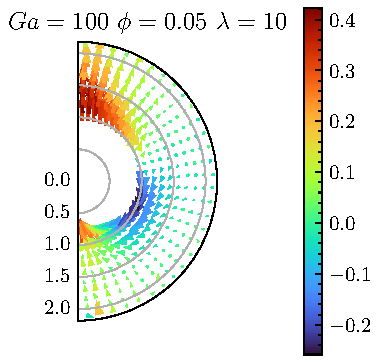
\includegraphics[height=0.35\textwidth]{image/HOMOGENEOUS_NEW/Dist/U_l_10_Ga_100_PHI_5.pdf}
    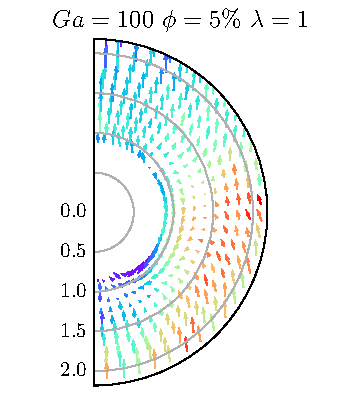
\includegraphics[height=0.35\textwidth]{image/HOMOGENEOUS_NEW/Dist/U_l_1_Ga_100_PHI_5.pdf}
    \caption{
         Quiver plots of the conditioned droplet velocity field $\textbf{u}^\text{r}(\textbf{x},\textbf{r},t)$ colored by the averaged dimensionless vertical velocity difference : $(\textbf{u}^\text{r}_p - \textbf{u}_p )/ \textbf{u}_p$, for $\phi = 0.05$ and $Ga = 100$. 
         (left) High viscosity ratio $\lambda = 10$.
         (right) Low viscosity ratio, $\lambda = 1$.
         }
    \label{fig:unst_l}
\end{figure}
On \ref{fig:unst_l} (left) we first note that $\textbf{u}^\text{r}(\textbf{x},\textbf{r},t)$ behave similarly to the low inertia case displayed on \ref{fig:unst_ga} (left).
However, for $\lambda = 10$, the isolated droplets' velocity is roughly equal to $\textbf{u}_p$. 
Note that the trace of \textbf{R} is rather high in this case, (see \ref{fig:A}). 
Thus, the majority of the droplets are rather isolated. 
Consequently, if the isolated droplets rise at the average velocity of the dispersed phase it is because most of them are isolated droplets.
Therefore, this fact is not particularly relevant as it is just a statistical bias. 
Nevertheless, we can still conclude that for $\lambda = 10$ droplets go faster with a nearest neighbor on top or bottom, while for  $\lambda = 1$ droplets go faster when the nearest neighbor is at a large distance. 

\subsubsection{Relation with the dispersed phase velocity fluctuation tensor}

In addition to providing physical explanations, the field $\textbf{u}_p^d = \textbf{u}^r_p - \textbf{u}_p$ is of great importance to study the droplet phase fluctuation tensor $\pavg{\textbf{u}_i' \textbf{u}_i'}$ which is of crucial importance in multiphase flow modeling. 
Indeed, it can be shown that 
\begin{equation}
    \frac{\pavg{ \textbf{u}_i' \textbf{u}_i'}}{n_p}(\textbf{x},t)
    =  
    \int_{\mathbb{R}^3 }
    \textbf{u}_p^d
    \textbf{u}_p^d
    P_{nst}(\textbf{r}|\textbf{x},t)
    d\textbf{r}
    + \int_{\mathbb{R}^3 }
    \textbf{F}(\textbf{r},\textbf{x},t)
    d\textbf{r}
    \label{eq:particle_center_of_mass_velocities}
\end{equation}
where, $\textbf{F} = \avg{\sum_i\sum_{j\neq i}\delta_j\delta_i h_{ij}(\textbf{u}_i - \textbf{u}_p^{nst})(\textbf{u}_i - \textbf{u}_p^{nst})}$. 
Thus, the ensemble-averaged dispersed phase Reynolds stress is the sum of the fluctuation given by $\textbf{u}_p^r$ plus an additional contribution from the other droplet velocity fluctuations around the average field $\textbf{u}_p^d$. 
At low volume fraction, it is reasonable to think that the former term represents the majority of the droplet phase fluctuation. 
Therefore, \ref{fig:unst_l} constitutes a visual representation of the droplet phase agitation tensor $\avg{\delta_i \textbf{u}_i' \textbf{u}_i'}$. 
Notably, we can remark on \ref{fig:unst_l}  that the droplet phase fluctuations tensor seems to be anisotropic. 
Indeed, more vertical velocity fluctuations than horizontal one is observed. 
This implies that the ``granular temperature'' $k_p = \pavg{ \textbf{u}_i' \cdot \textbf{u}_i'}/(2n_p)$ is probably not sufficient to model $\avg{\delta_i \textbf{u}_i' \textbf{u}_i'}$ in buoyant emulsions. 

Based on \ref{eq:particle_center_of_mass_velocities} we can compute the variance of the velocity of sedimenting suspensions of spherical droplets in Stokes and dilute regimes.
The method is quite similar than what is done in \citet{zhang2021ensemble} and \ref{chap:pseudoturbulence}. 
This idea will be pursued in a future study. 


\subsubsection{Discussion}
% \tb{
%     The field $\textbf{w}_p^r$ is useful for several reasons. 
%     As discussed it might serve to close equations such as \ref{eq:dt_R}. 
%     Or simply it provides us with clear physical explanation of what particles interaction look like. 
%     Also, we believe that it might be useful for coalesce kernels modeling. 

    
% }

From \ref{sec:Theory} we demonstrated that $\textbf{R}(\textbf{x},t)$ follows a transport equation where the tensor $\textbf{W}(\textbf{x},t)$ acts as a source term. 
This tensor might be expressed as the symmetric part of $\int_0^\infty \textbf{r} \textbf{w}_p^\text{r} P(\textbf{x},\textbf{r},t) da$. 
Thus, the trends of the $\textbf{w}_p^\text{r}(\textbf{x},\textbf{r},t) $ in terms of the position determine the value of $\textbf{W}(\textbf{x},t)$ and partly determine the final value of $\textbf{R}(\textbf{x},t)$. 
In many of the graphs, we observed that the vertical components of $\textbf{w}_p^\text{r}$ were negative when the vertical component of \textbf{r} was positive and vice versa. 
Consequently, $W_{yy}$ must be on average negative and $W_{xx}$ positive, which ultimately contributes to the value of $\textbf{R}(\textbf{x},t)$ and $\textbf{A}(\textbf{x},t)$ through \ref{eq:dt_R} and justifies the sign of $A_{xx}$ in \ref{fig:A}. 

In \ref{fig:phase} we display the values of $W_{xx}$ in terms of $Ga$ and $\phi$. 
These graphs provide us with a concise description of the relative kinematics. 
We recall that $\textbf{W}:\bm\delta = 0$ as we demonstrated in \ref{sec:Theory}, thus the value  $W_{xx}$ entirely determines $W_{yy}$ since the problem is symmetric. 
For example, we see that the highest dimensionless relative velocity position is reached for $Ga = 10$ and $\phi = 0.01$. 
This implies that, it is in the dilute regime and with relatively small inertial effects, that the particles have the fastest relative motions. 
\begin{figure}[h!]
    \centering
    % \begin{tikzpicture}[scale=0.8]
    %     \node (img) at (0,0) {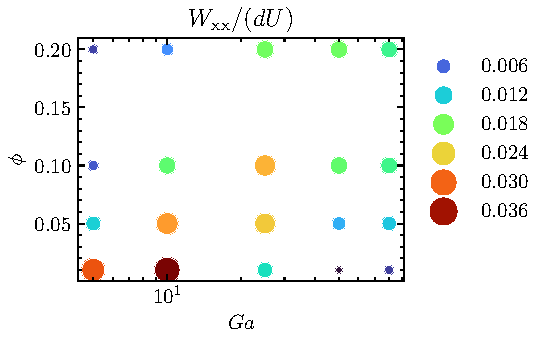
\includegraphics[height=5.5cm]{image/HOMOGENEOUS_NEW/PA/phase_Wxx_l_1.pdf}};
    %     \node (img) at (11,0) {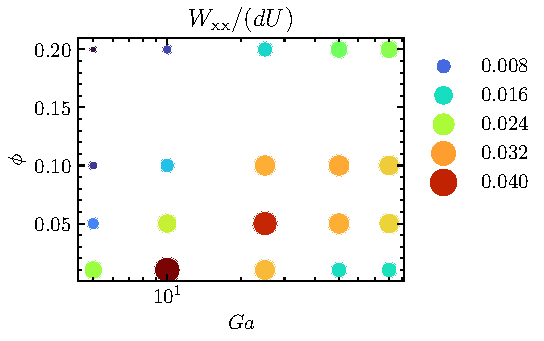
\includegraphics[height=5.5cm]{image/HOMOGENEOUS_NEW/PA/phase_Wxx_l_10.pdf}};
    % \end{tikzpicture}
    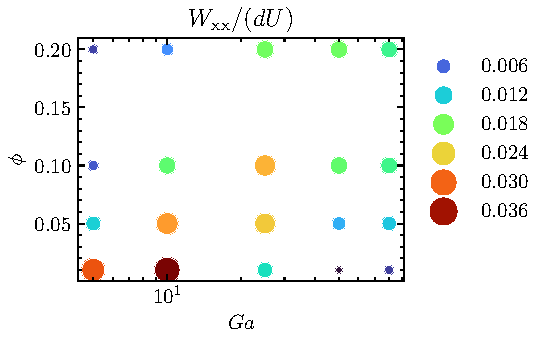
\includegraphics[height=5.5cm]{image/HOMOGENEOUS_NEW/PA/phase_Wxx_l_1.pdf}
    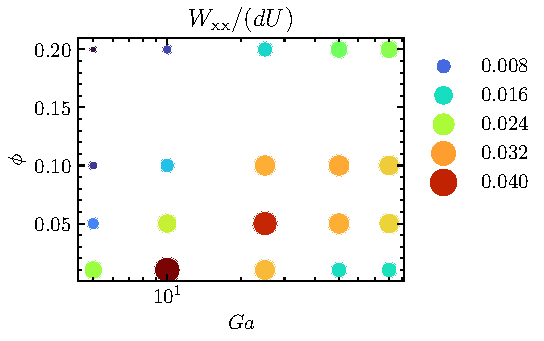
\includegraphics[height=5.5cm]{image/HOMOGENEOUS_NEW/PA/phase_Wxx_l_10.pdf}
    \caption{Phase diagram of the horizontal components of the dimensionless correlation tensor $W_{xx}/(Ud)$. 
        (left) Iso-viscous emulsion $\lambda = 1$.
        (right) Viscous droplets $\lambda = 10$ }
    \label{fig:phase}
\end{figure}
Is the relative velocity fields $\textbf{w}_p^r$ the cause of the microstructure shape as is suggested by \ref{eq:dt_R}. 
Or does $\textbf{w}_p^r$ the consequence of microstructure shape, as suggested by the previous graphs \eqref{fig:Why_Ga_matter,fig:Why_l_matter,fig:Why_Phi_matter} ?
Indeed, on \ref{fig:Why_l_matter} (right), the clear asymmetry with respect to the horizontal plane can be explained as the consequence of clusters in the flows. 
Although it is a complicated question, we believe that both are true, even if physical parameters also impact $\textbf{w}_p^r$, which makes the microstructure case dependent.  
Nevertheless, this makes $\textbf{W}(\textbf{x},t)$ potentially a function of $\textbf{R}(\textbf{x},t)$.
Depending on its relationship with $\textbf{R}(\textbf{x},t)$ this may modify the relaxation time.  
Thus, a more efficient way to close \textbf{W} in an objective manner would be to study the dynamic of interactions. 
In this work, we only provided kinematics   arguments to explain the microstructure shape. 
Of course to fully understand the physics of interaction one has to study the dynamics of interactions. 
It is in fact possible in our framework to include such dynamics variable by deriving an equation for \textbf{W} the same way we derived \ref{eq:dt_R} for \textbf{R}.
Thus work is still needed to fully understand interaction dynamics within this ``nearest-particle statistics'' framework. 



